\section{实验}
\label{sec:experiments}

\subsection{研究问题}

实验围绕以下问题展开：
\begin{itemize}
    \item \textbf{RQ1：}在动作完整的条件下，仅改变双臂相对时序是否足以显著改变任务结果？
    \item \textbf{RQ2：}敏感性是否随手臂、任务阶段和延迟强度呈现结构化差异，而非简单的单调退化？
    \item \textbf{RQ3：}用反事实成功样本和困难失败样本训练，是否优于相同规模的普通噪声增强？
    \item \textbf{RQ4：}在示范数量减少时，方法的相对收益是否更明显？
    \item \textbf{RQ5：}\todo{可选实机问题：仿真识别的敏感阶段与策略增益能否迁移到实机？}
\end{itemize}

为避免实验结束后再解释结果，我们预先给出与研究问题对应的可检验假设：
\begin{description}
    \item[H1（时序因果相关性）] 在累计动作不被删除的条件下，单臂相对延迟仍会使一部分基线成功轨迹转为失败；
    \item[H2（结构化敏感性）] 配对失败率同时依赖被干预手臂、干预阶段与延迟强度，并且不必随延迟单调变化；
    \item[H3（数据有效性）] 在相同源示范数和合成样本预算下，\method{} 的策略成功率高于 Random Delay 与 Positive Only；
    \item[H4（少样本优势）] 随源示范数量减少，\method{} 相对于 Source Only 的绝对提升增大。
\end{description}

\subsection{任务与数据划分}

主任务采用 DexMimicGen TwoArmThreading。该数据集包含 1025 条双臂示范和 218858 个时间步，控制频率为 20 Hz。\todo{增加 TwoArmTransport/TwoArmHandover 或另一个接触丰富任务，避免结论只依赖穿线任务。}

按源示范或初始状态簇划分训练、验证和测试集合，避免同一源轨迹的反事实版本跨集合泄漏。所有反事实必须在数据划分之后生成。少样本设置使用 $N\in\{5,10,25,50,100\}$ 条源示范，每个设置使用至少 3 个随机种子。模型选择只依据验证集，测试初始状态在方法定稿前固定并封存。

\begin{table}[t]
\centering
\caption{数据划分与用途。所有反事实仅由对应划分内的源轨迹产生。}
\label{tab:split}
\begin{tabular}{lcl}
\toprule
划分 & 比例/数量 & 用途 \\
\midrule
训练集 & 70\% & 生成反事实并训练策略 \\
验证集 & 15\% & 选择阈值、干预条件和模型检查点 \\
测试集 & 15\% & 仅用于最终策略评估 \\
敏感性筛选子集 & 训练集内50条 & 确定验证阶段的干预网格 \\
\bottomrule
\end{tabular}
\end{table}

\subsection{对比方法}

\begin{enumerate}
    \item \textbf{Source Only：}只使用原始少量示范；
    \item \textbf{Gaussian Noise：}在动作上加入高斯噪声，并保留仿真成功轨迹；
    \item \textbf{Global Time Warp：}两只手臂同步进行统一时间缩放；
    \item \textbf{Random Delay：}随机进行单臂延迟，不使用敏感性筛选和困难负样本；
    \item \textbf{Positive Only：}仅加入稳定成功的后缀延迟轨迹；
    \item \textbf{\method{}：}使用敏感性筛选的正样本和困难失败样本，并加入协同损失。
\end{enumerate}

所有方法使用相同基础策略、相同训练步数和相同增强样本预算，保证比较反映数据构造方式而非模型容量或数据数量差异。

\paragraph{公平性约束。}
Gaussian Noise、Global Time Warp 和 Random Delay 与本文方法具有相同的候选仿真次数；Positive Only 与完整方法具有相同的成功反事实数量；所有策略看到的成功动作监督条数保持一致。困难失败样本只进入协同判别损失，不作为行为克隆的目标动作。若某个基线的有效轨迹不足，则通过重复随机种子补齐候选预算，而不是重复已有轨迹。

\subsection{干预网格与两阶段实验协议}

为控制计算量，实验分为筛选和验证两个阶段。筛选阶段在训练集的50条示范上使用完整网格
\begin{equation}
e\in\{L,R\},\quad s/T\in\{0,0.25,0.5,0.75\},\quad
\delta\in\{2,4,6,10,15,20\}.
\end{equation}
根据配对失败率、任务距离和非冗余性选择2--3个代表性条件。验证阶段在完整训练集上只运行选定条件，防止根据测试结果反复挑选干预。延迟以控制步数和秒数同时报告。

\paragraph{训练协议。}
策略训练统一使用相同的观测、动作表示、网络结构、优化器和更新次数。反事实成功轨迹可进入行为克隆监督；困难失败轨迹只用于协同可行性判别，不把失败动作作为模仿目标。当前导出器已经生成 robomimic 兼容的 \texttt{obs/actions/next\_obs/rewards/dones} 字段及 stable-positive、hard-negative、invalid-negative 和 behavior-cloning 掩码，并完成单示范 BC 训练与闭环评估接口测试。该接口测试仅验证软件链路，不计入策略性能结果。

\subsection{评价指标}

\begin{itemize}
    \item 任务成功率与轨迹结束后的稳定成功率；
    \item 最小/最终任务距离，例如针尖到环中心的距离；
    \item 对未见初始状态、物体姿态和执行延迟的泛化成功率；
    \item 数据效率：达到给定成功率所需的真实源示范数量；
    \item 校准指标：协同判别头对困难失败的 AUROC、AUPRC；
    \item \todo{实机：每种方法至少20次独立试验，报告成功率和95\%置信区间。}
\end{itemize}

稳定成功率定义为
\begin{equation}
\mathrm{SSR}=\frac{1}{M}\sum_{i=1}^{M}\mathbb{I}\!\left[\text{轨迹执行结束并保持 }H\text{ 步后仍成功}\right].
\end{equation}
只在基线稳定成功的轨迹集合 $\mathcal{B}$ 上计算配对失败率
\begin{equation}
\mathrm{PFR}(c)=\frac{1}{|\mathcal{B}|}\sum_{i\in\mathcal{B}}
\mathbb{I}\!\left[y^{\mathrm{stable}}_{i,c}=0\right],
\end{equation}
从而避免把原本无法稳定复现的源轨迹归因于反事实干预。少样本数据效率另外用成功率—示范数量曲线下面积衡量。

\subsection{流程验证实验}

在大规模实验之前，我们选取3条示范进行了27个条件的端到端流程测试，包含左右臂、4/6步延迟以及轨迹起点/中点两种干预位置。表~\ref{tab:pilot}给出稳定成功率。3条基线都曾在轨迹中达到成功，但仅2条在额外保持10步后仍然成功，说明稳定性检查能够排除瞬时满足几何阈值的轨迹。

\begin{table}[t]
\centering
\caption{流程验证中的稳定成功率。$n=3$，括号内为只对2条稳定基线计算的配对成功率。该结果仅验证代码和指标，不用于支持论文假设。}
\label{tab:pilot}
\begin{tabular}{lccc}
\toprule
干预手臂 & 延迟步数 & 起点比例 & 稳定成功率（配对成功率） \\
\midrule
左臂 & 4 & 0.0 & 33.3\%（50.0\%） \\
左臂 & 4 & 0.5 & 33.3\%（50.0\%） \\
左臂 & 6 & 0.0 & 66.7\%（100.0\%） \\
左臂 & 6 & 0.5 & 66.7\%（100.0\%） \\
右臂 & 4 & 0.0 & 66.7\%（50.0\%） \\
右臂 & 4 & 0.5 & 100.0\%（100.0\%） \\
右臂 & 6 & 0.0 & 33.3\%（50.0\%） \\
右臂 & 6 & 0.5 & 33.3\%（50.0\%） \\
\bottomrule
\end{tabular}
\end{table}

该流程测试至少确认了三点：完整数据可重放、干预结果可按 demo 配对、成功判据对保持时间敏感。表中非单调现象只能作为后续完整实验的待检验观察，不能据此声称存在普遍的接触模式切换。

\subsection{50条示范的时序敏感性筛选}

我们随后在50条训练集示范上执行完整的$2\times4\times6$干预网格，共得到2450条基线或反事实轨迹。基线轨迹中49条曾在执行过程中满足成功条件，但只有35条在额外保持10个控制步后仍然成功。因此，后续配对分析固定在这35条稳定基线示范上，避免将源轨迹本身无法稳定复现错误归因于时序干预。

\begin{table}[t]
\centering
\caption{代表性时序干预条件的配对结果。PFR仅在35条稳定基线示范上计算，区间为Wilson 95\%置信区间。20 Hz控制频率下，2、10、20步分别对应0.10、0.50、1.00秒。}
\label{tab:screening}
\begin{tabular}{lrrr}
\toprule
干预条件 & 配对成功率 & PFR & PFR 95\% CI \\
\midrule
左臂，2步，75\%起点 & 85.7\% & 14.3\% & [6.3\%, 29.4\%] \\
右臂，10步，50\%起点 & 68.6\% & 31.4\% & [18.6\%, 48.0\%] \\
左臂，10步，0\%起点 & 54.3\% & 45.7\% & [30.5\%, 61.8\%] \\
左臂，20步，0\%起点 & 14.3\% & 85.7\% & [70.6\%, 93.7\%] \\
\bottomrule
\end{tabular}
\end{table}

最强干预条件为“左臂从轨迹起点延迟20步”，其配对失败率达到85.7\%；相同延迟量施加到右臂时，各阶段的配对失败率为34.3\%--48.6\%。这表明结果并非只由轨迹整体变慢解释，而与被延迟手臂及干预阶段有关。左臂2步延迟的配对失败率仅为14.3\%--22.9\%，随延迟增大总体上升；但各阶段内部并不严格单调。现阶段该非单调性只作为接触状态分析的对象，不将其直接解释为接触模式切换。

根据筛选结果，后续策略实验预先固定三类条件：左臂2步、75\%起点作为低破坏正样本候选；右臂10步、50\%起点作为中等难度边界条件；左臂20步、0\%起点作为困难失败条件。条件选择在策略测试前完成，后续不根据测试集成功率重新挑选。

\subsection{少样本策略接口诊断}

在正式多随机种子实验前，我们使用5条稳定源示范进行了单种子 BC-RNN 诊断。Source Only 使用5条基线轨迹；Positive Only 在相同源示范上加入9条逐轨迹验证为稳定成功的反事实。两者训练50个 epoch，并在20个未用于训练的初始状态上闭环执行300步。两种策略的稳定成功率均为0\%，说明该设置处于成功率地板区，不能用于判断数据增强的有效性。Source Only 与 Positive Only 的平均最小任务距离分别为0.3515和0.3401，但 Positive Only 仅在9/20个配对状态上更接近目标，平均最终距离还增加0.0030。因此这些距离差异只用于诊断，不作为方法收益。

该结果将正式实验顺序调整为：先在25或50条源示范上建立非零 Source Only 基线，再进行三随机种子方法比较；只有高数据量基线通过后，才回到5/10条示范验证少样本优势。这样可区分“增强无效”和“所有方法都尚未学会任务”两种情况。

进一步诊断表明，25条稳定源示范、100 epoch 的轻量状态 BC-RNN 在20个未见初始状态上仍为0\%成功，并且在5个训练初始状态上也为0\%成功。其教师强制开环动作 MSE 为0.0282，仅为零动作 MSE（0.1806）的15.6\%，说明网络学到了示范动作，但小的逐步误差在闭环中累积。将 LSTM 隐状态扩大到512维并训练200 epoch 后，训练轨迹复现仍为0/5；额外加入双臂关节位置、关节速度和夹爪速度后，训练损失降至0.0071，但复现率仍为0/5。由此可见，当前低维逐步 BC 不适合作为正式策略基线。

官方数据同时包含 agent view 和双腕相机三路$84\times84$图像。后续核心策略实验将采用与 DexMimicGen 官方协议一致的视觉 BC-RNN（或更强序列策略），而低维策略只保留为软件接口和地板效应诊断。上述0\%结果不进入主结果表，也不能用于判断反事实增强是否有效。

我们已进一步验证视觉训练链路：使用外部 HDF5 链接构造25条示范子集，在不复制原始4 GB图像数据的情况下成功加载三路相机、ResNet-18+SpatialSoftmax编码器和BC-RNN，并完成一次训练更新及模型保存。该实验仅证明数据与代码接口可用。当前本机PyTorch为CPU版本，正式视觉策略训练需迁移至GPU环境后再执行官方规模的训练协议。

\subsection{主结果表模板}

\begin{table}[t]
\centering
\caption{不同源示范数量下的策略成功率（\%）。报告均值$\pm$标准差。}
\label{tab:main}
\resizebox{\linewidth}{!}{
\begin{tabular}{lccccc}
\toprule
方法 & 5 demos & 10 demos & 25 demos & 50 demos & 100 demos \\
\midrule
Source Only & -- & -- & -- & -- & -- \\
Gaussian Noise & -- & -- & -- & -- & -- \\
Global Time Warp & -- & -- & -- & -- & -- \\
Random Delay & -- & -- & -- & -- & -- \\
Positive Only & -- & -- & -- & -- & -- \\
\method{} & \textbf{--} & \textbf{--} & \textbf{--} & \textbf{--} & \textbf{--} \\
\bottomrule
\end{tabular}}
\end{table}

\begin{table}[t]
\centering
\caption{反事实数据构成与计算成本。该表用于排除“更多计算或更多样本”带来的不公平优势。}
\label{tab:data_budget}
\begin{tabular}{lrrrr}
\toprule
方法 & 源示范 & 候选轨迹 & 入选轨迹 & 仿真小时 \\
\midrule
Random Delay & -- & -- & -- & -- \\
Positive Only & -- & -- & -- & -- \\
\method{} & -- & -- & -- & -- \\
\bottomrule
\end{tabular}
\end{table}

\subsection{反事实敏感性分析}

对每条示范分别改变干预手臂 $e$、起点比例 $s/T\in\{0,0.25,0.5,0.75\}$ 和延迟 $\delta$。绘制稳定成功率热图，并统计相对于基线成功示范的配对失败率。由于接触系统可能发生模式切换，不应预设成功率随延迟单调下降；应报告完整响应曲线，并结合接触图和任务距离解释非单调区间。

50条示范的完整筛选结果如图~\ref{fig:sensitivity_heatmap}所示。左臂长延迟区域形成明显的高失败带，而右臂响应整体较弱；这支持H1，并为H2中的手臂与阶段依赖提供初步证据。由于同一示范的多个条件彼此相关，正式验证仍需在预先固定条件上进行配对检验和多重比较校正；图中结果不用于证明策略学习收益。

\begin{figure}[t]
\centering
\IfFileExists{figures/sensitivity_heatmap.png}{
    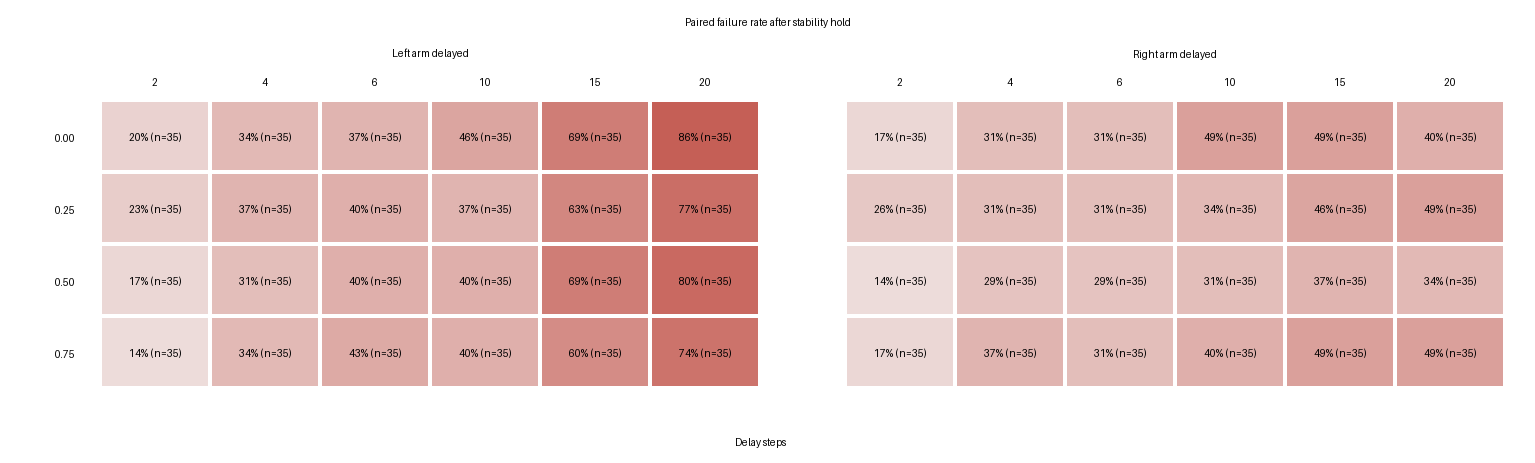
\includegraphics[width=\linewidth]{figures/sensitivity_heatmap.png}
}{
    \begin{tikzpicture}[x=1.05cm,y=0.62cm,font=\small]
        \draw[->] (0,0) -- (6.6,0) node[right]{延迟步数};
        \draw[->] (0,0) -- (0,5.7) node[above]{阶段};
        \foreach \x/\lab in {1/2,2/4,3/6,4/10,5/15,6/20}
            \node[below] at (\x,0) {\lab};
        \foreach \y/\lab in {1/0\%,2/25\%,3/50\%,4/75\%}
            \node[left] at (0,\y) {\lab};
        \foreach \x in {1,...,6}
            \foreach \y in {1,...,4}
                \draw[fill=gray!15] (\x-0.38,\y-0.32) rectangle (\x+0.38,\y+0.32);
        \node[align=center] at (3.5,5.1) {等待完整筛选结果；\\左右臂分别绘图};
    \end{tikzpicture}
}
\caption{协同敏感性热图。颜色表示稳定基线子集上的配对失败率，格内同时标注有效样本数。}
\label{fig:sensitivity_heatmap}
\end{figure}

\subsection{消融实验}

\begin{enumerate}
    \item 去除稳定保持检查，只使用轨迹中任意时刻成功；
    \item 用冻结窗口代替动作完整的后缀延迟，检验动作删除造成的混杂；
    \item 去除困难失败样本或去除协同判别损失；
    \item 不按敏感性筛选，随机选择等量反事实；
    \item 改变延迟集合、阶段数量、保持步数和每条源示范的样本预算；
    \item 在 BC-RNN、ACT 和 Diffusion Policy 上替换基础策略，检验方法的模型无关性。
\end{enumerate}

\subsection{统计检验}

策略评估使用固定测试初始状态并进行配对比较。成功率报告 bootstrap 95\% 置信区间；同一初始状态下的二元成功结果使用 McNemar 检验；多随机种子结果同时报告均值和标准差。涉及多个干预条件时使用 Benjamini--Hochberg 方法控制错误发现率。默认显著性水平设为 $0.05$，bootstrap 重采样10000次。除显著性外同时报告绝对成功率差和置信区间，避免只依赖 $p$ 值。

\subsection{失败模式分析}

除成功率外，随机抽取并人工复核失败轨迹，将其归入以下类别：未建立关键接触、接触建立过早或过晚、支撑手失稳、物体滑移、发生非目标碰撞、到达任务区域但保持后退出。对每类至少展示一个基线—反事实配对案例，并报告不同方法的失败构成。该分析用于回答性能变化是否确实来自协同时序，而不是控制器数值不稳定或仿真异常。
